
% LaTeX Template for short student reports.
% Citations should be in bibtex format and go in references.bib
\documentclass[a4paper, 11pt]{article}

\usepackage[top=3cm, bottom=3cm, left = 2cm, right = 2cm]{geometry} 
\geometry{a4paper} 
\usepackage[utf8]{inputenc}
\usepackage{textcomp}
\usepackage[spanish]{babel}
\usepackage{graphicx} 
\usepackage{amsmath,amssymb}  
\usepackage{bm}  
\usepackage[pdftex,bookmarks,colorlinks,breaklinks]{hyperref}  
%\hypersetup{linkcolor=black,citecolor=black,filecolor=black,urlcolor=black} % black links, for printed output
\usepackage{tocloft}

\hypersetup{%
  colorlinks = true,
  linkcolor  = black
}

\usepackage{memhfixc} 
\usepackage{pdfsync}  
\usepackage{fancyhdr}
\usepackage{amsmath}

\usepackage{listings}
\usepackage{xcolor}

\usepackage{tikz}

\usepackage{smartdiagram}  

\usepackage{url}

\usepackage{etoolbox,refcount}
\usepackage{multicol}

\usepackage{graphicx}
\usepackage{subcaption}
\usepackage{matlab-prettifier}
\usepackage{chemmacros}
\renewcommand\lstlistingname{Código}
\renewcommand\lstlistlistingname{Códigos}
\newcounter{countitems}
\newcounter{nextitemizecount}
\newcommand{\setupcountitems}{%
  \stepcounter{nextitemizecount}%
  \setcounter{countitems}{0}%
  \preto\item{\stepcounter{countitems}}%
}
\makeatletter
\newcommand{\computecountitems}{%
  \edef\@currentlabel{\number\c@countitems}%
  \label{countitems@\number\numexpr\value{nextitemizecount}-1\relax}%
}
\newcommand{\nextitemizecount}{%
  \getrefnumber{countitems@\number\c@nextitemizecount}%
}
\newcommand{\previtemizecount}{%
  \getrefnumber{countitems@\number\numexpr\value{nextitemizecount}-1\relax}%
}
\makeatother    
\newenvironment{AutoMultiColItemize}{%
\ifnumcomp{\nextitemizecount}{>}{3}{\begin{multicols}{2}}{}%
\setupcountitems\begin{itemize}}%
{\end{itemize}%
\unskip\computecountitems\ifnumcomp{\previtemizecount}{>}{3}{\end{multicols}}{}}

\definecolor{codegreen}{rgb}{0,0.6,0}
\definecolor{codegray}{rgb}{0.5,0.5,0.5}
\definecolor{codespurple}{rgb}{0.58,0,0.82}
\definecolor{backcolour}{rgb}{0.95,0.95,0.92}

\lstdefinestyle{mystyle}{
    backgroundcolor=\color{backcolour},   
    commentstyle=\color{codegreen},
    keywordstyle=\color{magenta},
    numberstyle=\tiny\color{codegray},
    stringstyle=\color{codepurple},
    basicstyle=\ttfamily\footnotesize,
    breakatwhitespace=false,         
    breaklines=true,                 
    captionpos=b,                    
    keepspaces=true,                 
    numbers=left,                    
    numbersep=5pt,                  
    showspaces=false,                
    showstringspaces=false,
    showtabs=false,                  
    tabsize=2
}

\lstset{style=mystyle}


\graphicspath{ {images/} }

\begin{document}
\selectlanguage{spanish}

\begin{titlepage}
  \clearpage\thispagestyle{empty}
  \centering
  \vspace{1cm}
  % Rubriker
  {\Huge \textbf{Centro de Investigación y Estudios Avanzados del I.P.N.} \par}
  \vspace{1cm}

  \begin{figure}[h!]
    \centering
    
\includegraphics[scale=0.5]{cinves.png}
  \end{figure}
    
  \vspace{1cm}
  {\Huge \textbf{Reconocimiento de 8 herramientas}\par} 
  \vspace{4cm}
  {\Large Materia: Análisis de Imágenes Digitales \par} 
  \vspace{3cm}
  {\Large Catedrático: Dr. Wilfrido Gómez-Flores \par} 
  \vspace{1cm}
  {\Large Alumno: Luis Alberto Ballado Aradias \par} 
  
  \vspace{3cm}
  % Datum
  {\normalsize \today \par}
  %  \pagebreak
\end{titlepage}

\tableofcontents{}

\pagebreak
\renewcommand\lstlistlistingname{Lista de códigos}
\lstlistoflistings

\renewcommand{\listfigurename}{Lista de figuras}
\listoffigures

\pagebreak
\section{Introducción}

El Análisis de Imágenes Digitales es un área fascinante que engloba muchas áreas de las ciencias computacionales como Optimización y Aprendizaje de máquinas.\\

El procesamiento de imágenes es un área multidisciplinaria que tiene como objetivo la manipulación y análisis de la información de una imagen en su parte más reducida conocida como pixel (picture element). Emergiendo una gran cantidad de técnicas y metodologías para el procesamiento y manipulación de imágenes.\\

Con el aumento de imágenes digitales, el procesamiento se ha vuelto necesario para aplicaciones como en robótica, que la segmentación de imágenes puede facilitar la navegación para un robot aéreo \cite{smolyanskiy2017lowflying}, en el diagnóstico de cáncer ayuda a los médicos en dar diagnósticos más acertados \cite{10059977}. Asimismo, en la parte del entretenimiento con implementación de realidad aumentada \cite{8776989} .\\

La detección y reconocimiento que son parte del área de visión por computadora, se han vuelto cada vez más utilizadas en aplicaciones como traductores de idiomas, análisis médicos, reconocimiento de rostros faciales.\\

La detección y categorización de objetos con imágenes se descompone de los siguientes procesos:

\begin{enumerate}
\item \textbf{Adquisición de la imagen.-} La toma de fotografía se realiza mediante una cámara  que cuente con un sensor que puede ser de tipo CMOS, el sensor convierte la captura de la escena en señales digitales que son guardadas como una imagen.
\item \textbf{Preprocesamiento.-} Mediante las técnicas existentes se busca el mejoramiento del contraste, realzar características reduciendo el ruido, para hacer de la imagen lo más limpia posible para el paso de segmentación. 
\item \textbf{Segmentación.-} Es la obtención de las regiones de interés que ayuda a la extracción de características. Ésta imagen binaria debe tomar la silueta de la figura lo más aproximada posible.
\item \textbf{Extracción de características.-} Éste proceso busca describir en cierta forma la imagen, describiendo valores de forma geométrica, colores, texturas y valores invariantes que se mantienen a pesar de rotaciones o escalamientos.
\item \textbf{Clasificación.-} Asigna una clase a cada región de interés dentro de la imagen basados en los rasgos extraidos en el paso anterior.
\end{enumerate}

El proyecto busca el reconocimiento de ocho herramientas, aplicando las técnicas vistas en clase con el uso de MATLAB.\\

La figura \ref{etapas_basicas} muestra las etapas a desarrollar para el reconocimiento de las ocho herramientas.\\

\begin{figure}[h]
\centering

\includegraphics[width=0.7\textwidth]{etapas_basicas}
\caption{Etapas básicas para el análisis de imágenes.}
\label{etapas_basicas}
\end{figure}

Una imagen $f(x,y)$ se puede modelar como el producto de dos componentes $f(x,y) = i(x,y),r(x,y)$, donde $0<i(x,y)<\infty$ es la componente de iluminación y $0<r(x,y)<1$ es la componente de reflactancia.\\

Las dificultades que se tienen dentro del procesamiento de imágenes digitales son la iluminación del ambiente, siendo los sensores perceptibles a la iluminancia al obtener la imagen.\\

%Las operaciones aritméticas entre pixeles, la adición de la misma imagen por varias iteraciones puede ayudar a la reducción de ruido, sustracciones de dos imágenes de la misma toma, puede ayudar a detectar movimientos, la multiplicación de imágenes para enmascarar zonas de interés.\\

%En la información que puede obtener de sus vecinos para detectar bordes a partir de distancias entre pixeles, siendo una de ellas la distancia euclidiana $D_{e}(p,q)=[((x-u)^{2}+(y-v)^{2})^{\frac{1}{2}}]$ \\

%cuatro vencindad usando los vecinos horizontales y verticales.\\

%Suponga una imagen con k regiones disjuntas $R_{k}, k=1,2,..,k$ sea $R_{u}$ la unión de las k regiones y $(R_{u})^{c}$ su complemento.\\

%Entonces los puntos en Ru representan el primer plano y los puntos de $(R_{u})^{c}$ representan el fondo.\\






%Se probó la detección de bordes a partir del gradiente, pero la demaciada información nos afectaba en un ciclo para detectar bordes como canny edges.\\

%EJEMPLO DE LAPLACIANO DEL GAUSIANO\\

%Los beneficios de la aplicación del teorema de convolución nos ayuda en la reducción de la complejidad computacional, al solo considerar una multiplicación en  frecuencia.\\

%Operadores morfologicos\\



\section{Adquisición de la imagen}

La adquisición de las imágenes se realizó con las siguientes herramientas:

\begin{itemize}
\item Cámara web Logitech C920s HD Pro 1080p webcam 
\item Cubo para la toma de fotografías marca Puluz, ver figura \ref{cubo}
\item Control de iluminación dimmer, ver figura \ref{dimmer}
\end{itemize}

\begin{figure}[ht]
\centering
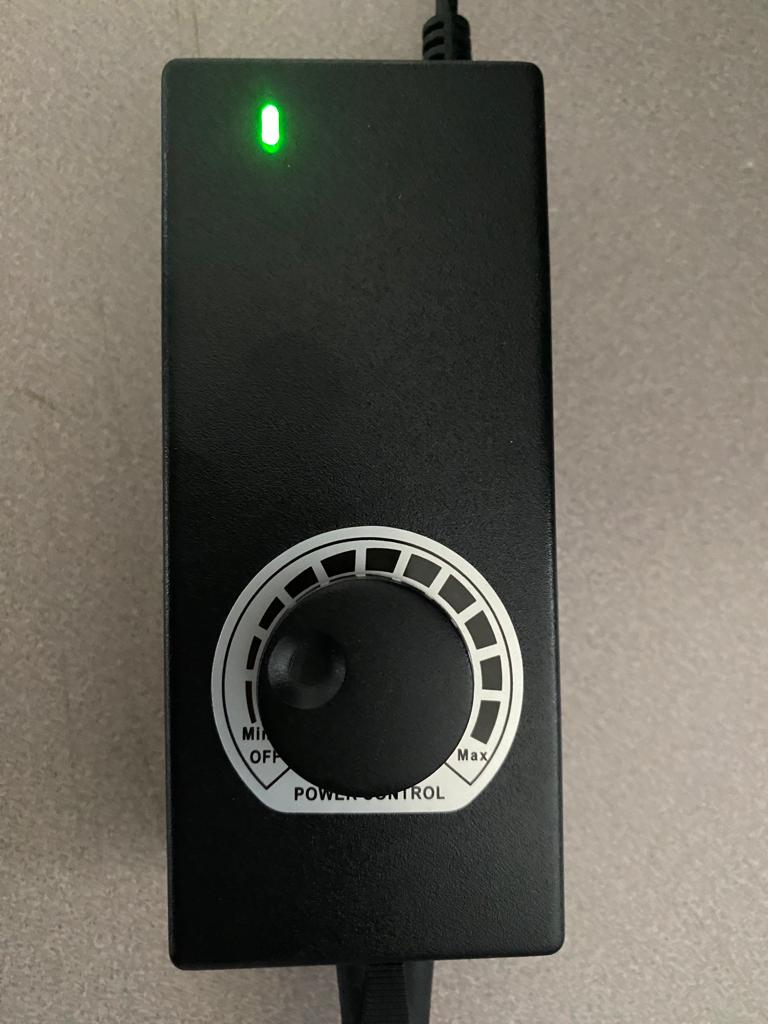
\includegraphics[width=0.4\textwidth]{dimer1}
\caption{Dimmer para el ajuste de la iluminación.}
\label{dimmer}
\end{figure}

La cámara web cuenta con un sensor de tipo CMOS de 2-mega pixel \cite{camara}, obteniendo imágenes limpias y muy bien contrastadas.\\

El objetivo del proyecto, es el reconocer automáticamente ocho herramientas que son:

\begin{AutoMultiColItemize}
\item Martillo
\item Desarmador
\item Cinta de medir
\item Llave perica
\item Tijeras
\item Pinza de punta
\item Pinza eléctricas
\item Pinza de presión
\end{AutoMultiColItemize}

La toma de fotografías se realiza en un ambiente controlado como se muestra en la figura \ref{cubo}, ajustando la iluminación con un dimmer mostrado en la figura \ref{dimmer}.

\begin{figure}[ht]
\centering
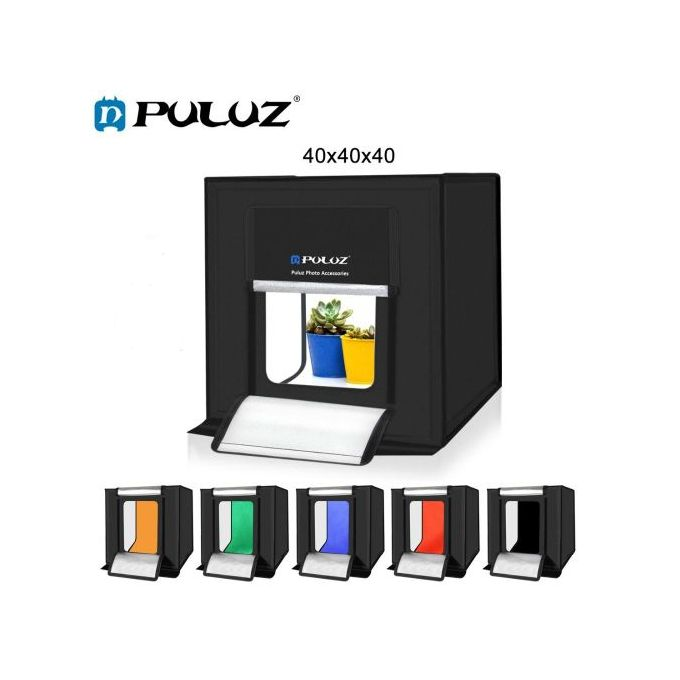
\includegraphics[width=0.6\textwidth]{cubo}
\caption{Cubo para la adquisición de imágenes.}
\label{cubo}
\end{figure}

Se usaron transformaciones geométricas para modificar la relación espacial entre píxeles en una imagen, usando propiedades que no deformen al objeto de interés como:

\begin{itemize}
\item Rotaciones
\item Traslaciones
\end{itemize}

Logrando crear imágenes artificiales, de manera que sirvan para el aumento del conjunto de imágenes.\\

\pagebreak
\section{Preprocesamiento}

Al contar con imágenes de buena calidad, solo se mejoró el contraste para reducir las sombras que las herramientas pueden formar y lograr obtener el contorno que representa más la imagen a reconocer.\\

El mejoramiento es la manipulación de una imagen, de tal forma que el resultado sea más útil que la imagen original para una aplicación en particular.\\

Una transformación de intensidad nos ayuda a modificar el constraste. Dentro del proyecto se aplicó una transformación de intensidad con un escalar de 1.5, para algunas imágenes más obscuras el valor de 2 resulta mejor para la detección de bordes más cercanos al objeto.\\

\begin{figure}[ht]%
    \centering
    \subfloat[\centering Imagen original]{{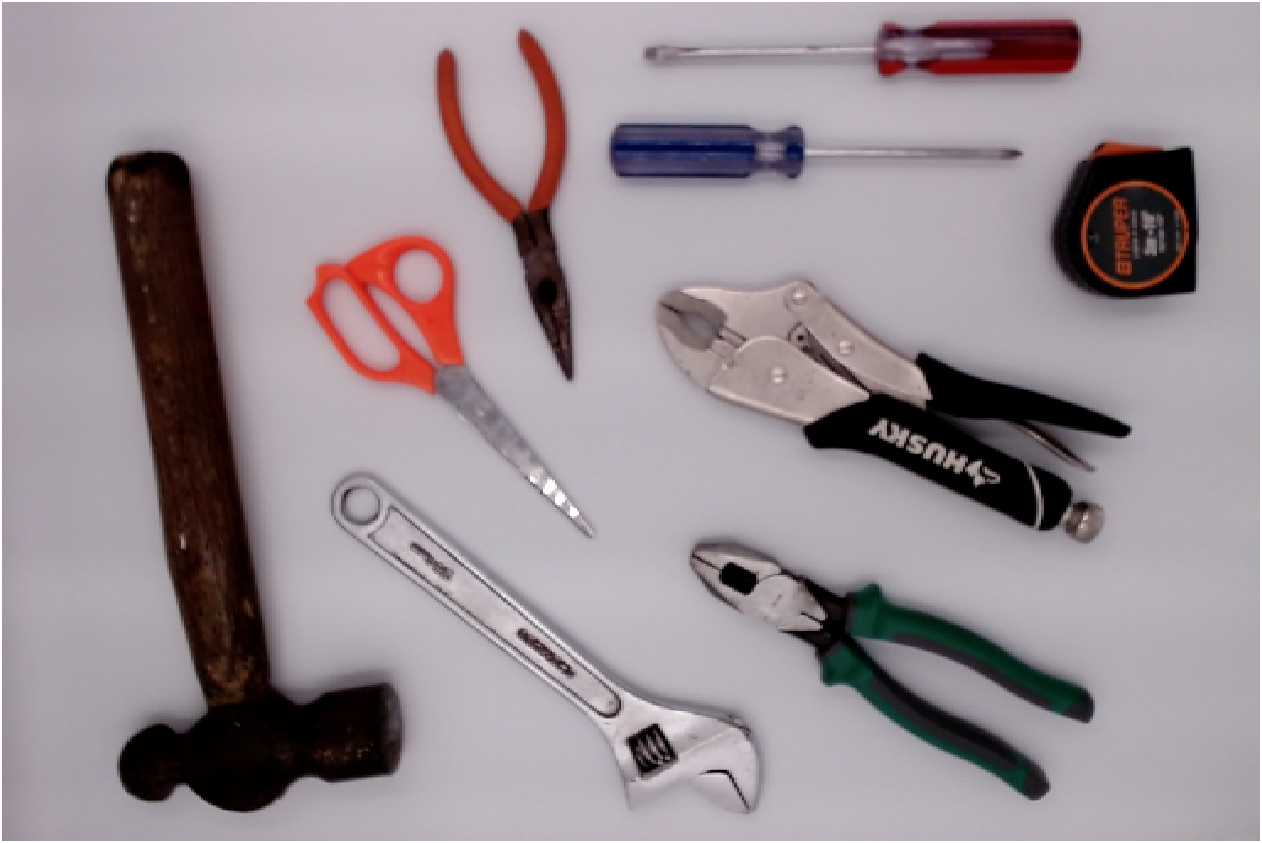
\includegraphics[width=7cm]{paso1} }}%
    \qquad
    \subfloat[\centering Imagen modificada del brillo]{{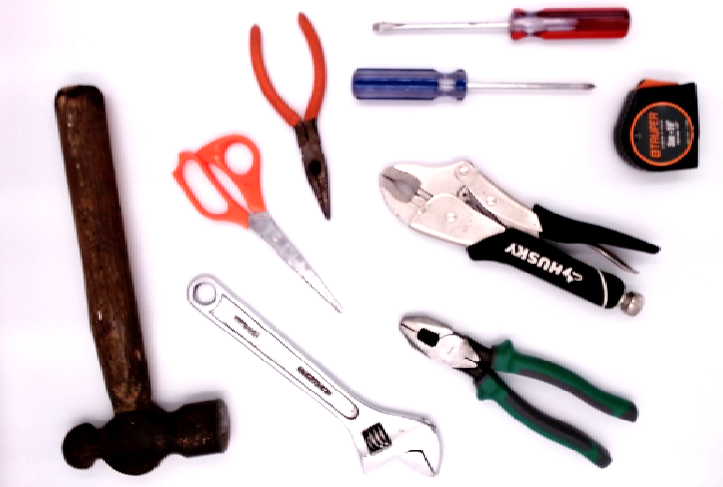
\includegraphics[width=7cm]{brillo} }}%
    \caption{Mejoramiento de contraste.}%
    \label{fig:grayImage}%
\end{figure}

De esta forma pudimos darle un alto contraste a la imagen como se puede apreciar en la figura \ref{fig:grayImage}.\\

A partir de la imagen original pasada a double\footnote{se hace un cambio de estructura a double}, esta imagen se multiplica por un escalar de brillo para tener la imagen con el brillo alto.

\begin{lstlisting}[style=Matlab-editor, caption=Factor de brillo]
  %% pasar a double
  original_gris = double(I);
  %% multiplicar por el factor de ruido
  img_ajustada = original_gris * factor_brillo;
\end{lstlisting}

A pesar de que los objetos en su mayoría poseen partes cromadas, se logran contrastar con el fondo original blanco. Logrando apreciar mejor los objetos, este paso es de gran ayuda. Siendo el factor de brillo un atributo dentro de la función de segmentación.
%Ecualización del histograma.\\

%No se tuvo que ecualizar ni mejorar por CLAHE, pero es bueno saber la existencia de estas técnicas para crear sistemas y filtros sofisticados.\\

%Modo de degradación de una imagen.\\

%No se hizo uso de ningun filtro, buscando evitar el efecto de deslavado y poder detectar los bordes lo más puros posibles.\\

%Pero el filtro de difusión anisotrópico puede considerarse en la implementación.\\
\pagebreak
\section{Segmentación}

Se hacen pruebas con diversas técnicas de segmentación, optando por un resultado sencillo con uso de operaciones morfológicas en base a una imagen de detección de bordes con Canny Edges.\\

De igual forma se exploraron otras técnicas que se listan a continuación.\\

\begin{itemize}
\item Método de umbralado global \textbf{Método de Otsu}

  Éste método sería el indicado, pero las partes color cromo en los objetos afecta en el umbralado de la imagen, haciendo perder rasgos representativos de los objetos como las puntas en la tijera, las partes metálicas del desarmador o de las pinzas. La figura \ref{otsu} ilustra el resultado después de aplicar éste método (Otsu).
  
  \begin{figure}[ht]%
    \centering
    \subfloat[\centering Imagen original escala de grises]{{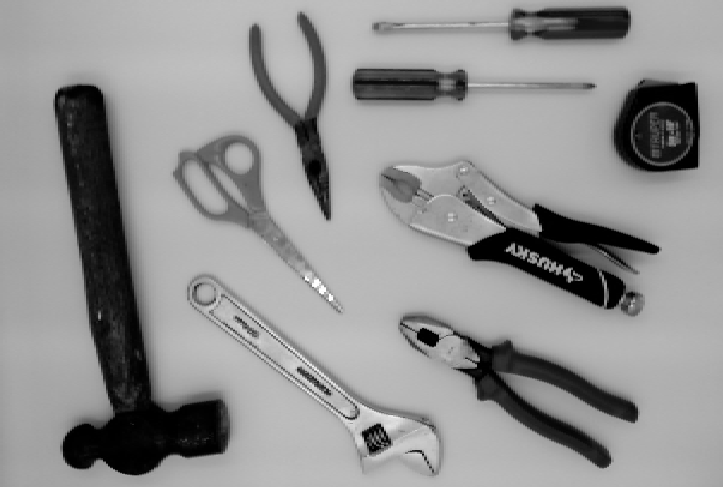
\includegraphics[width=7cm]{gris} }}%
    \qquad
    \subfloat[\centering Imagen umbralada con el método de otsu]{{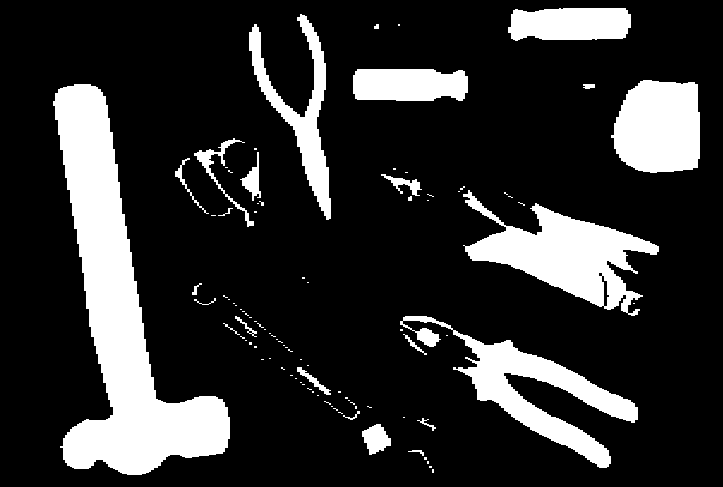
\includegraphics[width=7cm]{otsu} }}%
    \caption{Umbralado con método de otsu.}%
    \label{otsu}%
\end{figure}
  
\item Método de segmentación con \textbf{K-Means} (K-Means clustering)

  El algoritmo k-means es una técnica de agrupamiento que divide un conjunto de datos en k grupos o clusters. Los datos se agrupan de modo que los puntos de un grupo sean más similares que los puntos de otros grupos.\\
  
  A partir de una simple idea de crear dos grupos, el fondo y los objetos. Éste método sirve igual de bien que el Método de Otsu, pero en nuestro caso, el problema con el color cromo de los objetos hace que los valores cromo formen parte del conjunto del fondo. La figura \ref{kmeans} ilustra el resultado después de aplicar éste método (K-Means clustering).
  
  \begin{figure}[ht]%
    \centering
    \subfloat[\centering K-Means con dos clases]{{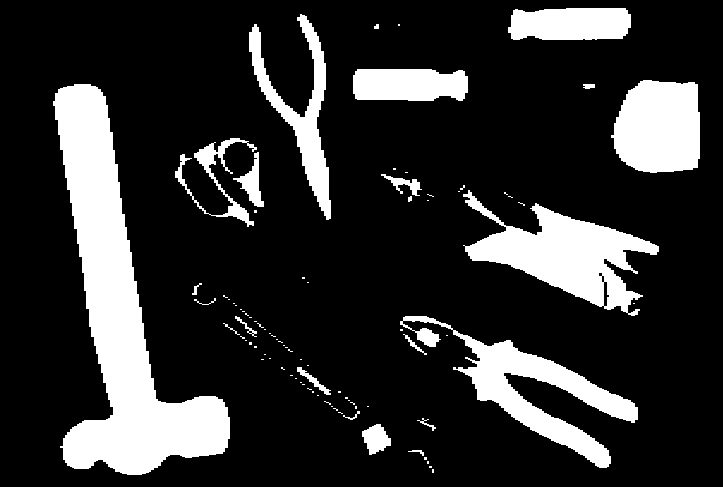
\includegraphics[width=7cm]{kmeans2} }}%
    \qquad
    \subfloat[\centering K-Means con tres clases]{{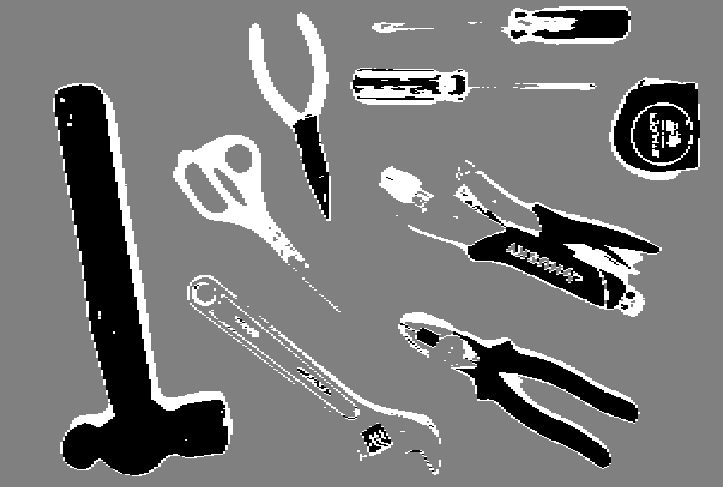
\includegraphics[width=7cm]{kmeans3} }}%
    \caption{Umbralado con K-Means.}%
    \label{kmeans}%
\end{figure}
  
\item Visualización de la \textbf{Entropía}

  Con una segmentación mediante el método de entropía se puede obtener la información de la presencia de los objetos, lamentablemente al estar con mucha información no fué utilizada en el proyecto. Pero replanteandolo nuevamenta, se puede hacer algun filtro para quedarse solo con los píxeles blancos con algun método como lógica difusa. La figura \ref{entropia} ilustra el resultado después de aplicar éste método (Entropía).

  \vspace{1cm}
  
  \begin{figure}[ht]%
    \centering
    \subfloat[\centering Imagen original escala de grises]{{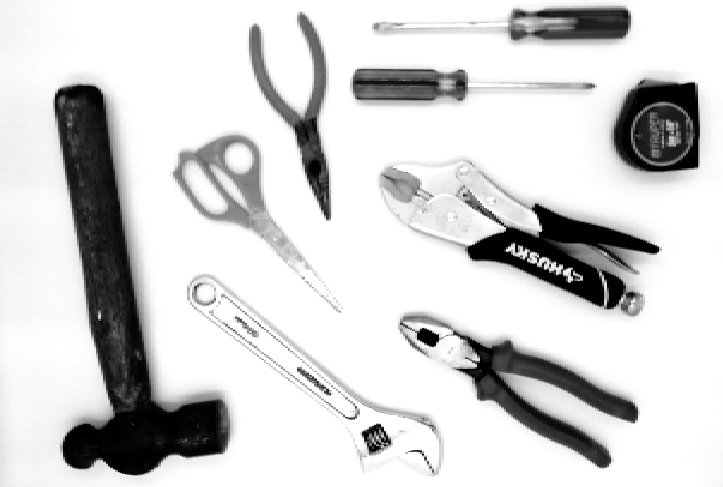
\includegraphics[width=7cm]{gris_entropia} }}%
    \qquad
    \subfloat[\centering Imagen después del método de entropía]{{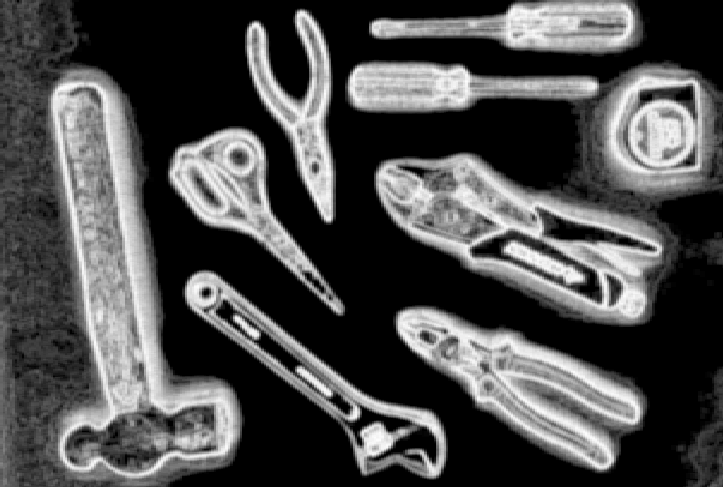
\includegraphics[width=7cm]{entropia} }}%
    \caption{Umbralado con método de entropía.}%
    \label{entropia}%
  \end{figure}

\item Detección de bordes \textbf{Canny Edges}\\

  Al contar con una representación limpia de los objetos de interés, la detección de los objetos a partir de sus bordes es una buena opción para lidear con las piezas cromadas. La figura \ref{canny} ilustra el resultado después de aplicar éste método.\\

  Probablemente sea el algoritmo para detección de bordes más usado para reconocer bordes en visión por computadora.\\

  Usa las mejores propiedades del operador del gradiente y el operador laplaciano. Básicamente los pasos que sigue son los siguientes:

  \begin{itemize}
  \item Suaviza la imagen con un filtro gausiano 2D
  \item Calcula el gradiente de la imagen usando un operador de sobel de 3x3, dando resultados de las derivadas para cada punto para el eje x y el eje y
  \item A partir de esos valores se puede calcular la magnitud para cada píxel, así como su orientación
  \item Se calcula el Laplaciano a lo largo de la dirección del gradiente
  \item Se usan los cruces por cero en el Laplaciano para encontrar la ubicación del borde
  \end{itemize}
  
  \begin{figure}[ht]%
    \centering
    \subfloat[\centering Imagen original escala de grises]{{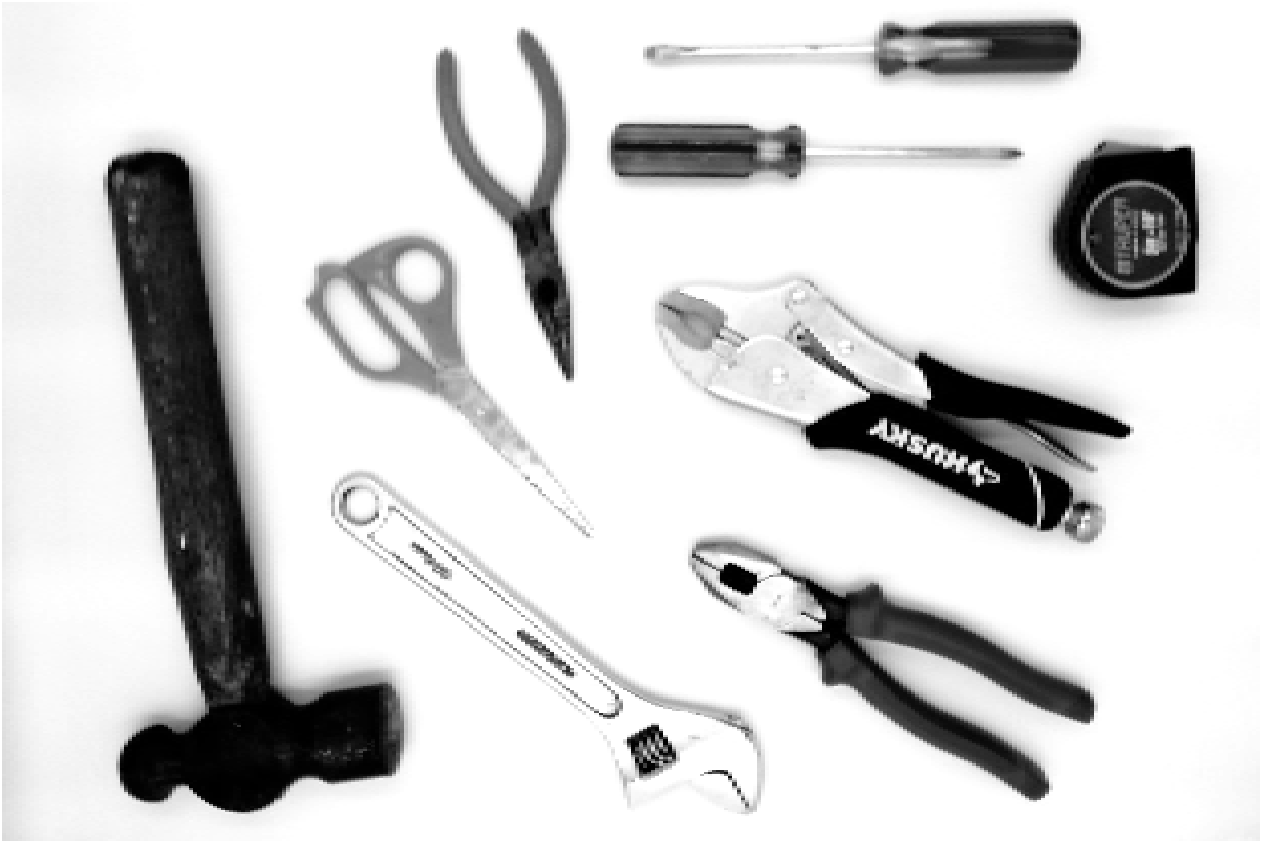
\includegraphics[width=7cm]{paso2} }}%
    \qquad
    \subfloat[\centering Detección de bordes con canny edges]{{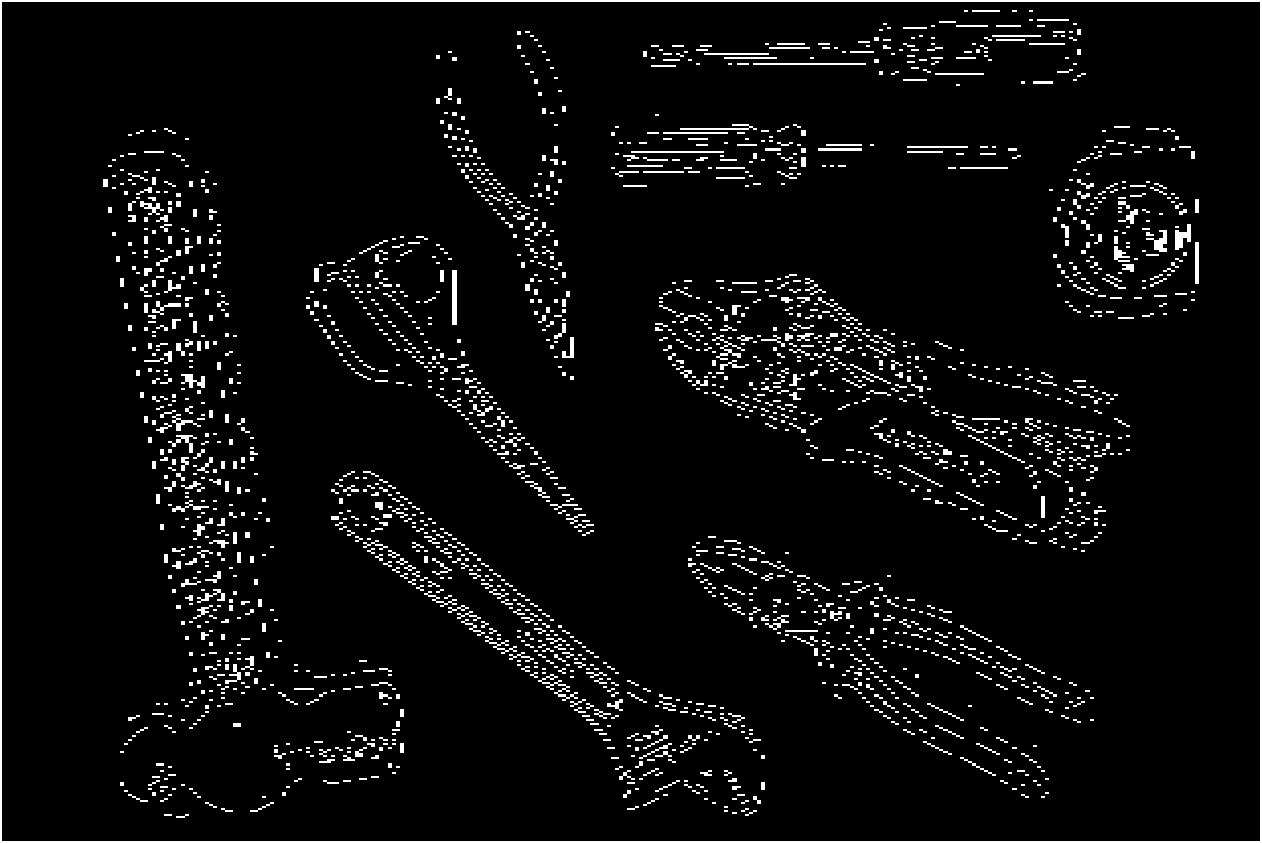
\includegraphics[width=7cm]{paso3} }}%
    \caption{Detección de bordes con canny edges.}%
    \label{canny}%
  \end{figure}
  
\end{itemize}

En matlab, el filtro de \textbf{Canny Edges} detecta bordes buscando los máximos locales del gradiente de la imagen. Las funciones de borde utilizan la derivada de un filtro gaussiano para calcular el gradiente. Este método utiliza dos umbrales para detectar bordes fuertes y débiles e incluye bordes débiles en la salida si están asociados con bordes fuertes. Debido a que el método de Canny utiliza dos umbrales diferentes, es menos propenso a errores debido al ruido que otros métodos y es más probable que detecte bordes realmente débiles \cite{canny}.

\begin{itemize}
\item Sigma valor escalar que especifica la desviación estándar del filtro gaussiano. El valor predeterminado es sqrt(2).  automáticamente en función de sigma \cite{canny}.

\item Umbral de sensibilidad es especificado como escalar numérico, la función en matlab ignora todos los bordes cuya intensidad no es mayor que threshold indicado, al no indicar un valor la función escoge los valores automáticamente \cite{canny}.
\end{itemize}

Al considerar la última técnica con la obtención de los bordes, debemos cerrar la imagen con elementos estructurantes, donde podemos encontrar la línea, ésta puede tomar valores de inclinacion a ciertos grados y ser de 4 ó 8 vecindad.\\

\subsection{Operaciones morfológicas}

La erosión y dilatación, operadores que fueron aplicados en el proyecto.

\begin{itemize}
\item Apertura: una erosión seguida de una dilatación $f \circ b = (f \fminus b) \fplus b$
\item Cerradorua: una dilatación, seguida de una erosión $f \bullet b = (f \fplus b) \fminus b$
\end{itemize}

El borde de un conjunto A que contiene los píxeles del primer plano se obtiene como:

\[B(A) = A - (A \fminus b)\]

donde A es la figura binaria y b el elemento estructurante.

\subsection{Erosión y dilatación}

Explicar las partes de erosion y dilatacion

\subsection{Rellenado de orificios}

Un orificio es una región del fondo rodeado por un borde conexo de pixeles del primer plano.\\

Se efectua una reconstrucción por dilatación.\\

Contorno de una región\\

El contorno de una región conexa es el conjunto de pixeles que tienen al menos en pixel vecino que corresponde al fondo en 4 ó 8 adyacencia.\\


Buscar que tipo de etiquetado usa BWLABEL .- QUE ALGORITMO?\\

Etiquetado de regiones conexas\\


\pagebreak
\section{Extracción de características}

El reconocimiento automático de objetos requiere calcular rasgos que describan propiedades fisicas de los objetos.\\

Un rasgo (atributo o característica), es un valor numérico que cuantifica alguna propiedad de forma, textura, color, geometria, etc.

\begin{itemize}
\item Un rasgo debe ser discriminante, invariante, incorrelado y rápido de computar.
\item Los rasgos de forma generalmente se calculan a partir de la segmentación del objeto y se divide entre todos los pixeles de las regiones de interés.
\item Basados en región distribución de todos los pixeles.
\item Basados en contorno, variaciones a lo largo del contorno.
\end{itemize}

La extracción de características que se utilizaron en el proyecto son las siguientes:

\begin{enumerate}
\item Rasgos geométricos básicos
\item Momentos de Hue
\item Cerco convexo 
\item Esqueletización
\end{enumerate}

\subsubsection{Geométricas básicas}

El área es el número total de pixeles que cubre la región del objeto.\\

El perimetro es la longitud del contorno del objeto. El resultado depende del tipo de conectividad que pueda tener. (4 ó 8 vecindad).

Para el cálculo de rasgos geométricos básicos, se hace uso del área y perimetro de la figura, el cual se obtiene mediante la imagen segmentada iterando entre todas las etiquetas.

\begin{figure}[ht]%
    \centering
    \subfloat[\centering Tijera]{{
\includegraphics[width=7cm]{tijera} }}%
    \qquad
    \subfloat[\centering Pinza de punta]{{
\includegraphics[width=6.3cm]{ppunta} }}%
    \caption{Imágenes segmentadas para obtención de rasgos geométricos básicos.}%
    \label{entropia}%
\end{figure}

\begin{AutoMultiColItemize}
\item Redondez
\item Circularidad
\item Compacidad
\item Factor de forma
\end{AutoMultiColItemize}

\newpage
\subsubsection{Rasgos basados en esqueleto}

Otra generación de rasgos usada en el proyecto, son los rasgos por esqueletizar la imagen.

\begin{figure}[ht]%
    \centering
    \subfloat[\centering Imagen umbralada]{{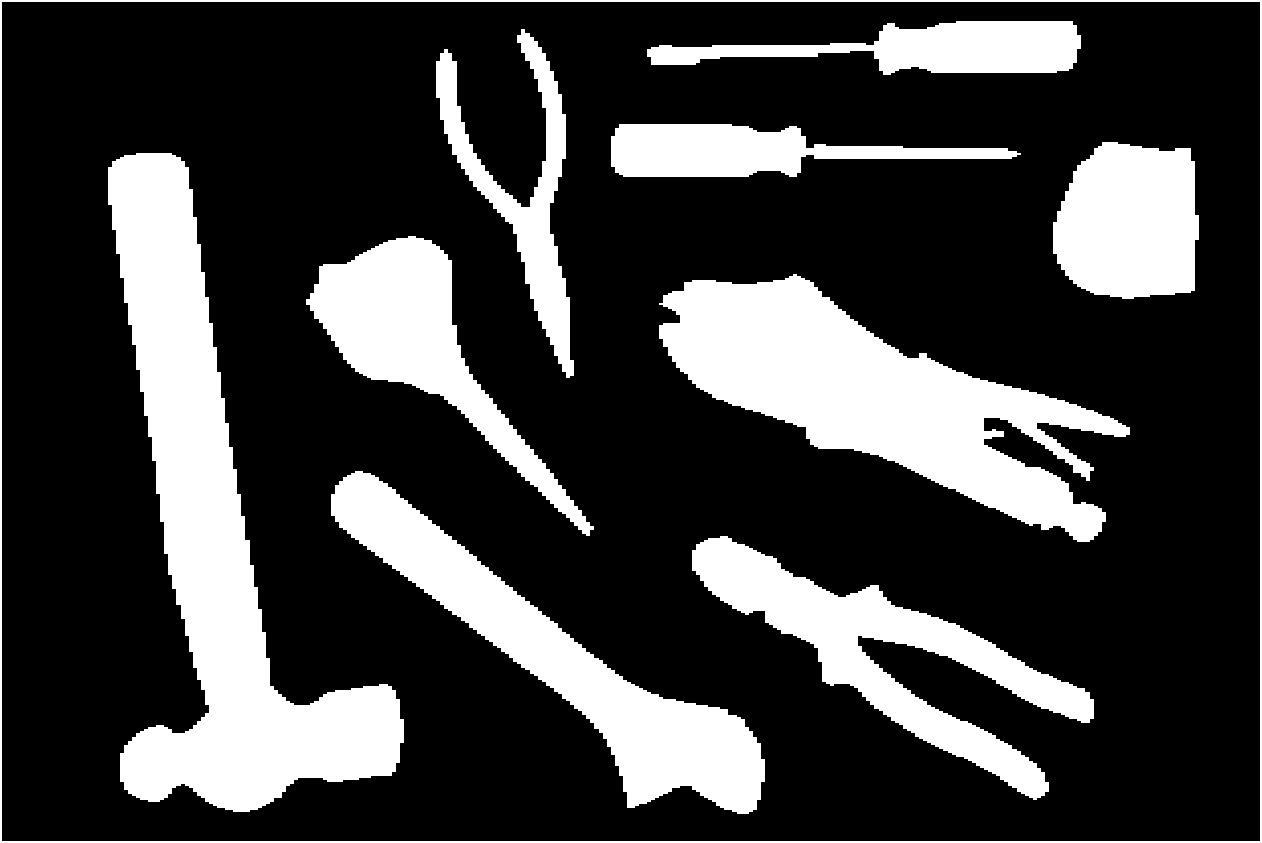
\includegraphics[width=7cm]{paso9} }}%
    \qquad
    \subfloat[\centering Imagen esqueletizada]{{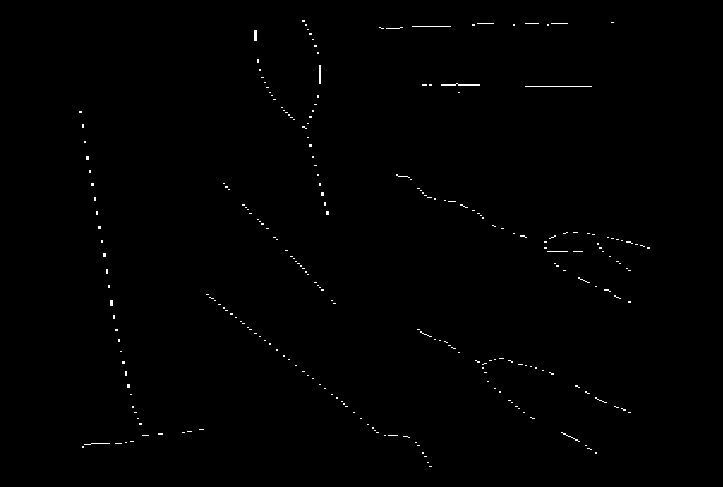
\includegraphics[width=7cm]{resultado_esqueleto} }}%
    \caption{Rasgos basados en esqueleto.}%
    \label{entropia}%
\end{figure}

\begin{itemize}
\item Puntos finales
\item Ramas
\item Número de pixles
\item Área
\item Perímetro
\end{itemize}

\subsubsection{Momentos invariantes Hue}

Los momentos son proyecciones de una función sobre una base polinomial usados para medir la distribución de masa de un cuerpo.

\subsubsection{Cerco convexo}

Los momentos son proyecciones de una función sobre una base polinomial usados para medir la distribución de masa de un cuerpo.

\begin{figure}[ht]%
    \centering
    \subfloat[\centering Imagen segmentada martillo]{{
\includegraphics[width=4cm]{martillo} }}%
    \qquad
    \subfloat[\centering Cerco convexo martillo]{{
\includegraphics[width=4cm]{cerco_convexo_martillo} }}%
    \caption{Rasgos cerco convexo.}%
    \label{entropia}%
\end{figure}

\begin{figure}[ht]%
    \centering
    \subfloat[\centering Imagen original escala de grises]{{
\includegraphics[width=6cm]{cerco_convexo_perica} }}%
    \qquad
    \subfloat[\centering Imagen después del método de entropía]{{
\includegraphics[width=4cm]{perica} }}%
    \caption{Umbralado con método de entropía.}%
    \label{entropia}%
\end{figure}


\begin{AutoMultiColItemize}
\item Solidez
\item Convexidad
\end{AutoMultiColItemize}

\pagebreak
\section{Clasificación}

Recordando las etapas del reconocimiento de objetos en imágenes.

\begin{enumerate}
\item Sensado.- Capturar la imagen.
\item Preprocesamiento.- Mejorar la calidad de la imagen y segmentar los objetos de interés.
\item Extracción de características.- Describir los objetos con rasgos cuantitativos discriminantes e invariantes.
\item Clasificación.- Asignar una etiqueta de clase a cada objeto.
\end{enumerate}

Obtener un vector de patrones.

Para el proyecto se consideran ocho clases sindo representadas por los objetos siguientes:

\begin{AutoMultiColItemize}
\item Martillo
\item Desarmador
\item Cinta de medir
\item Llave perica
\item Tijeras
\item Pinza de punta
\item Pinza eléctricas
\item Pinza de presión
\end{AutoMultiColItemize}

En este proyecto se usa el método de datos de entrenamiento que son vectores de patrones asociados a una etiqueta de clase (x,y) con $y \in \Omega = {w_{1},...,w_{c}}$\\

La selección del algoritmo de clasificación debe tener las siguientes cualidades.

\begin{itemize}
\item Generación de fronteras de decisión no lineales.
\item Clasificación en más de dos clases (multiclases).
\item Entrenamiento en un tiempo de cómputo razonable. 
\end{itemize}

Se elige el clasificador k-nn de vecinos más cercanos por su simpleza.\\

De modo que el reconocimiento de un objeto se realiza mediante la comparación entre el objeto de entrada y las muestras que se hayan obtenido en la etapa de extracción de características.\\
Al pasar por su segmentación y analizar los rasgos obtenidos, se asigna al grupo de mayor parecido. Entonces, el objeto cercano indica que son parecidos y la similitud se reducirá a medida que no tenga una similitud.\\

Diferentes distancias se pueden implementar en el algoritmo de los k-vecinos más cercanos, siendo la distancia euclidiana la que se utilizó en el desarrollo del proyecto. El parámetro k de vecinos, es el número de muestras de entrenamiento cercanas con las que se comparan.\\

El algoritmo KNN realiza los siguientes pasos:

\begin{enumerate}
\item Medir la distancia Euclidiana entre el objeto de interés y las muestras obtenidas la extracción de rasgos.
\item Identificar los patrones k más cercanos y obtener la etiqueta de la clase a la que pertenece.
\item Asignación de la clase al objeto de interés.
\end{enumerate}

\newpage
\section{Resultados}

\begin{figure}[h]
  \centering
  \begin{subfigure}{0.5\linewidth}
    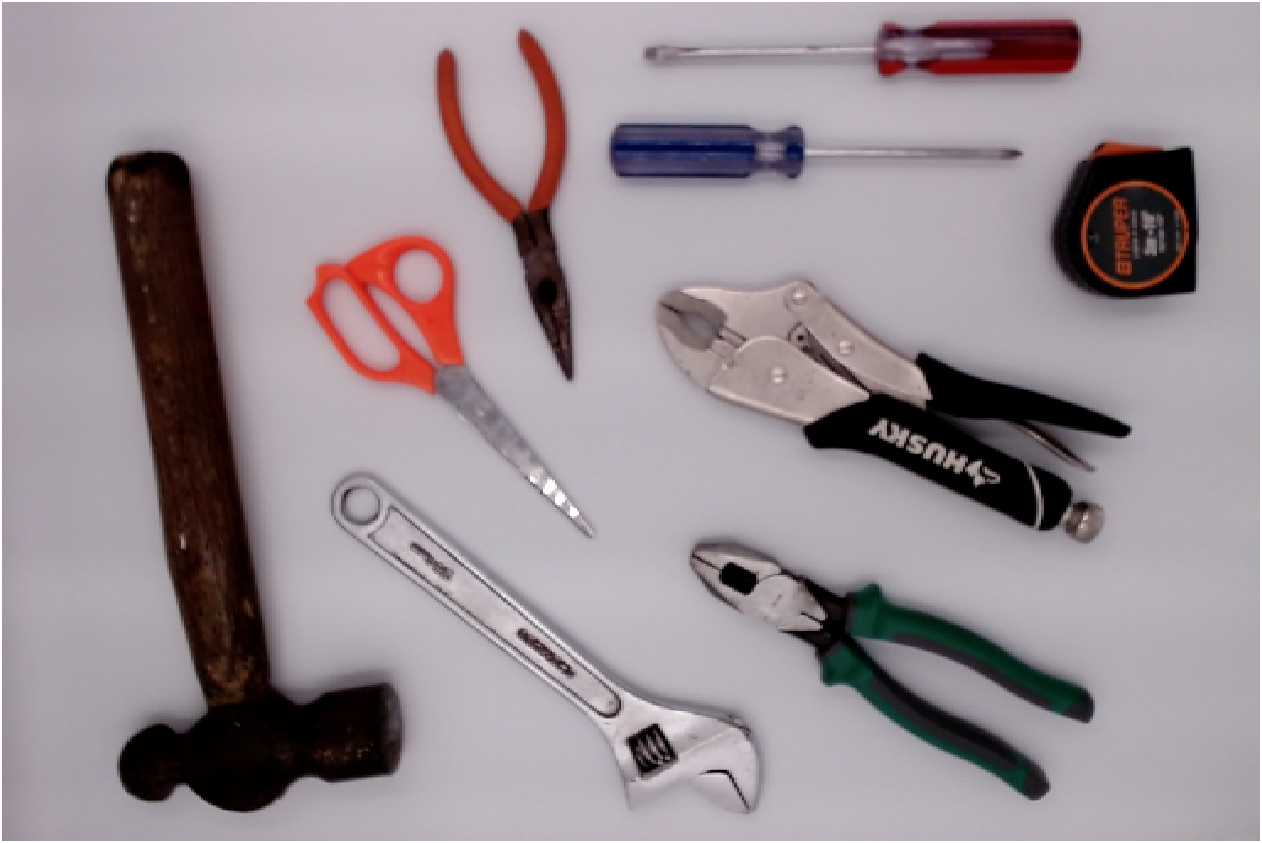
\includegraphics[width=\linewidth]{paso1} 
    \caption{Imagen Original}
    \label{fig:1a}
  \end{subfigure}\hfill
  \begin{subfigure}{0.5\linewidth}
    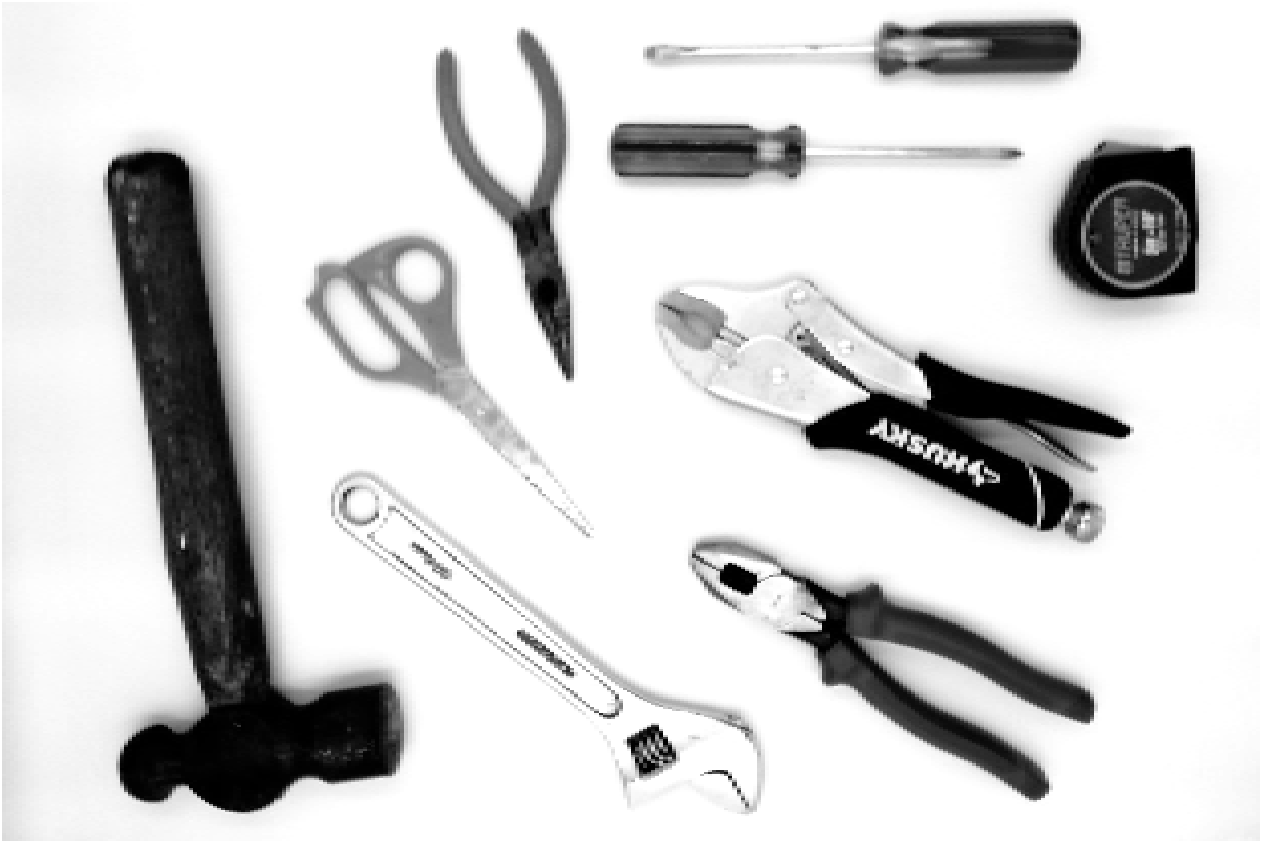
\includegraphics[width=\linewidth]{paso2}
    \caption{Imagen multiplicada por un escalar de brillo}
    \label{fig:1a}
  \end{subfigure}
  
  \begin{subfigure}{0.5\linewidth}
    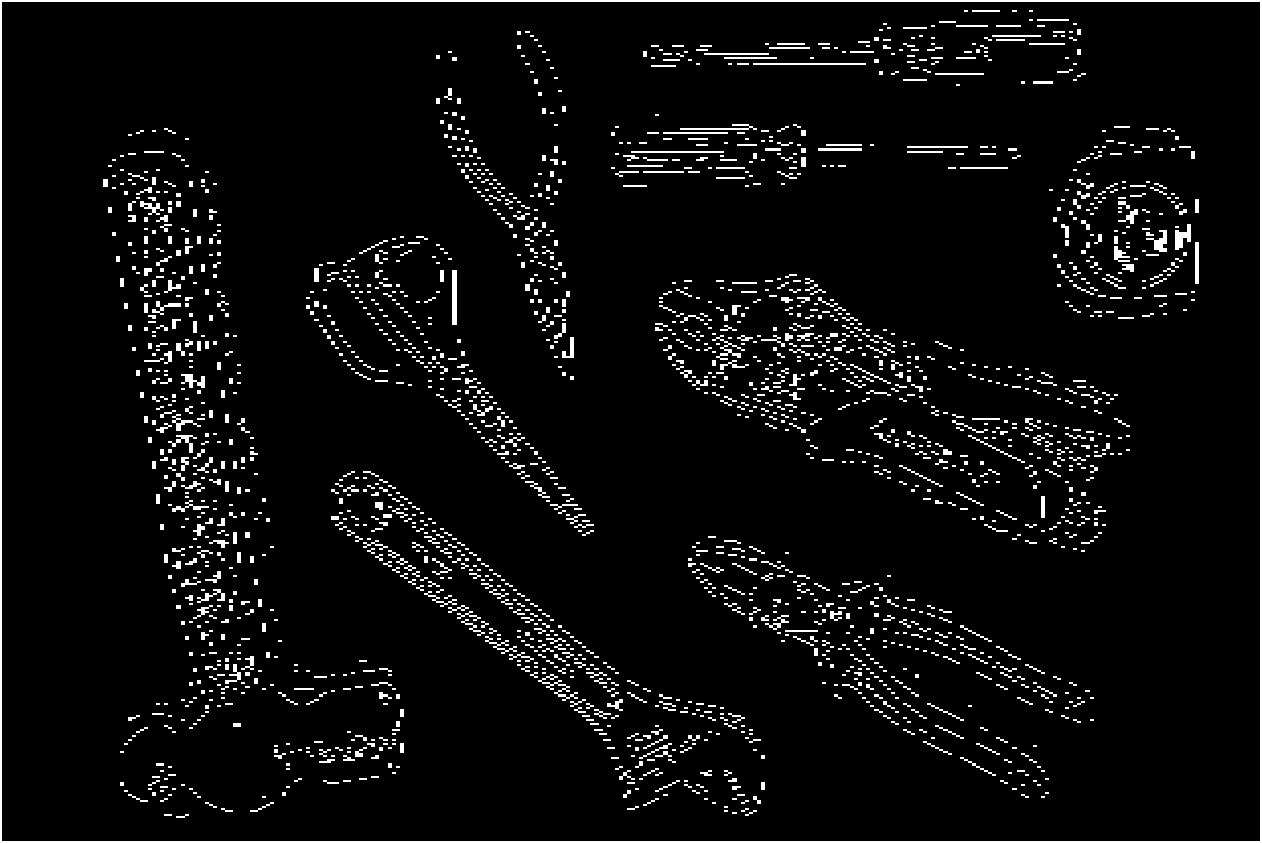
\includegraphics[width=\linewidth]{paso3}
    \caption{Imagen con detección de bordes canny edges}
    \label{fig:1a}
  \end{subfigure}\hfill
  \begin{subfigure}{0.5\linewidth}
    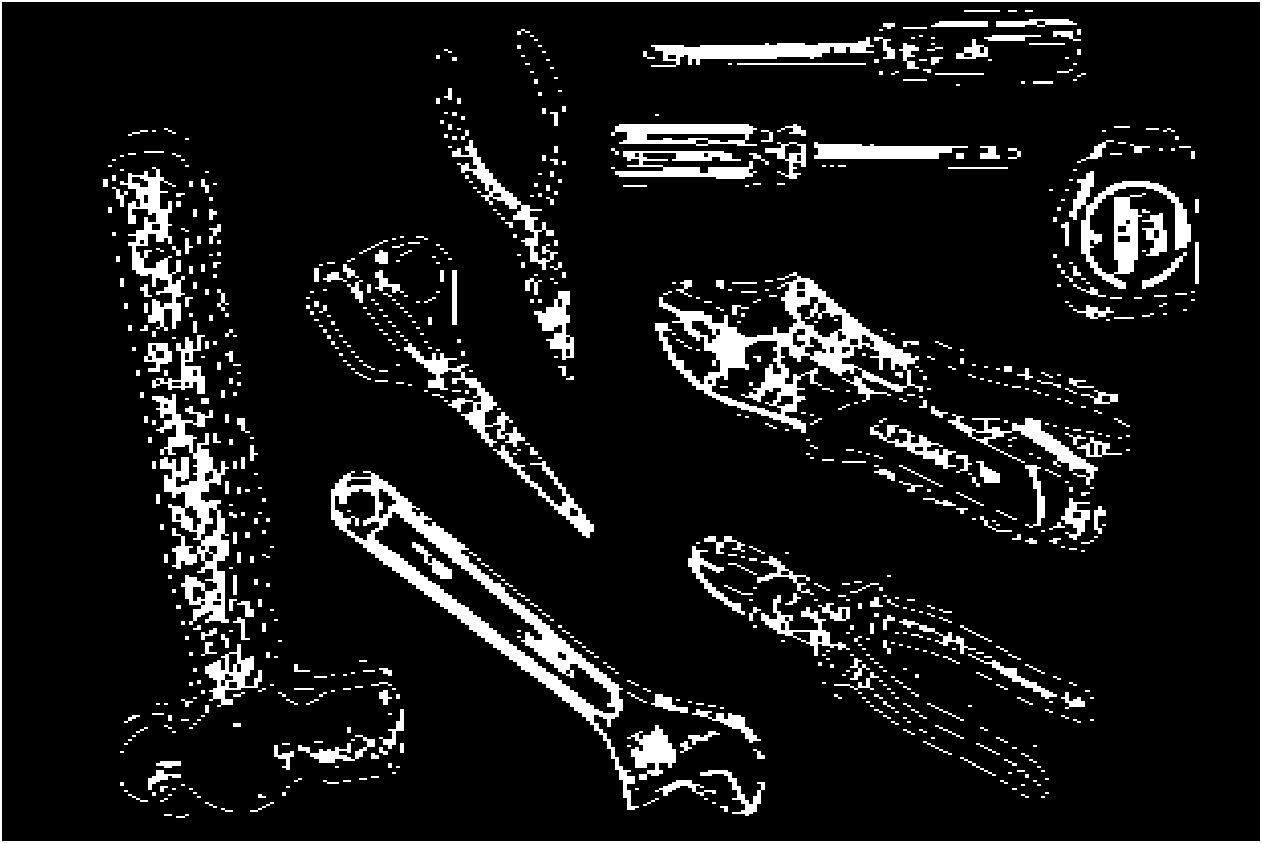
\includegraphics[width=\linewidth]{paso4}
    \caption{Llenando huecos con imfill}
    \label{fig:1a}
  \end{subfigure}
  \caption{Proceso de segmentado primera parte.}
  \label{fig:1}
\end{figure}

\begin{figure}[h]
  \centering
  \begin{subfigure}{0.5\linewidth}
    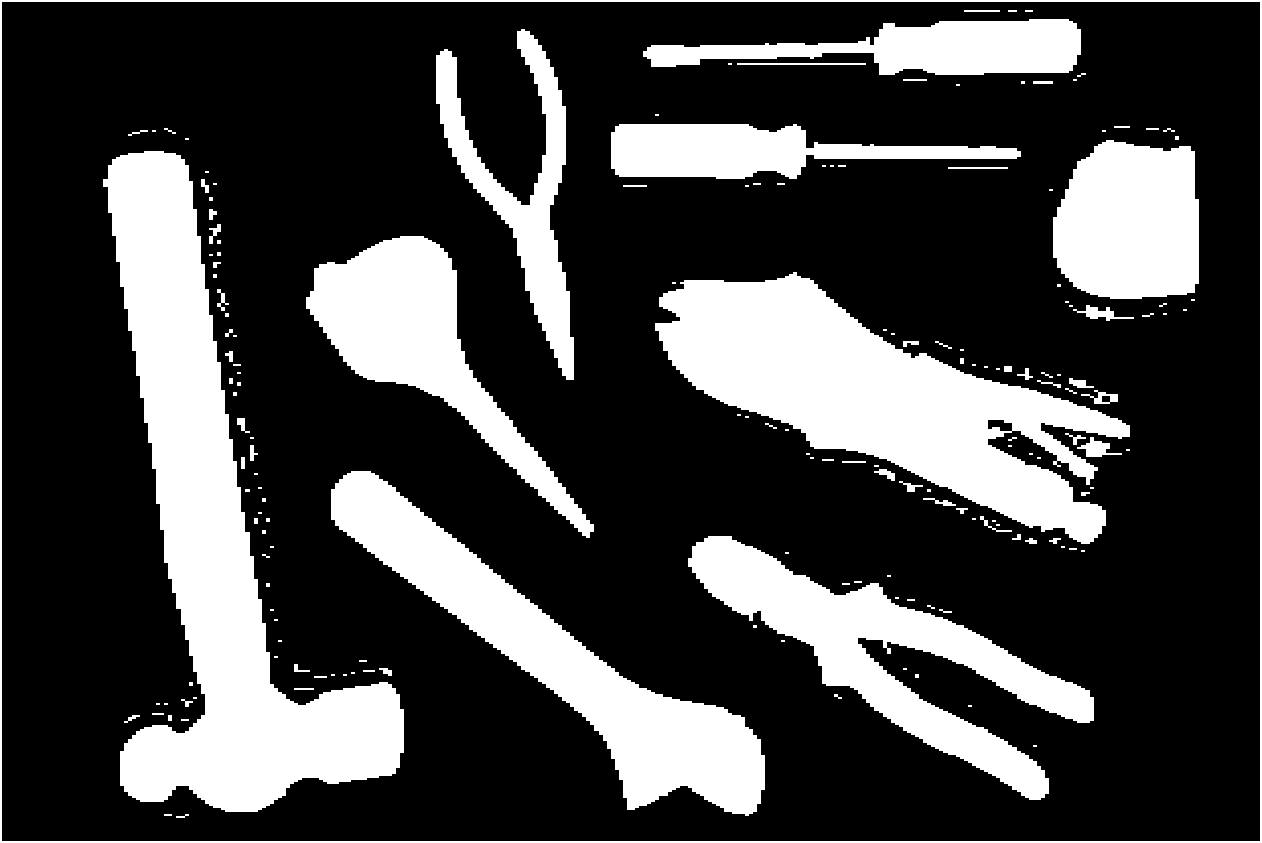
\includegraphics[width=\linewidth]{paso5} 
    \caption{Cerrar la imagen ,llenar huecos y limpiar imagen}
    \label{fig:1a}
  \end{subfigure}\hfill
  \begin{subfigure}{0.5\linewidth}
    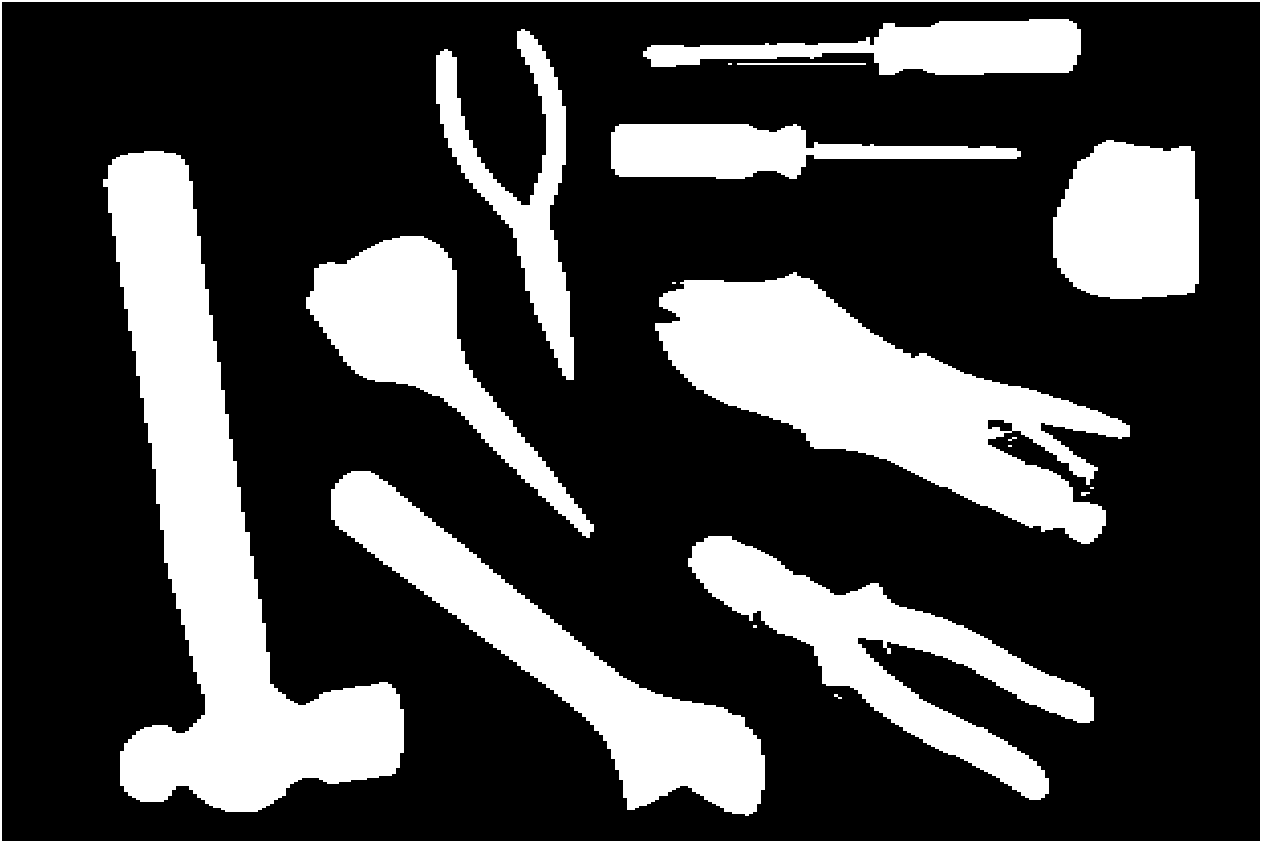
\includegraphics[width=\linewidth]{paso6}
    \caption{Erosión, seguida de una dilatación }
    \label{fig:1a}
  \end{subfigure}
  
  \begin{subfigure}{0.5\linewidth}
    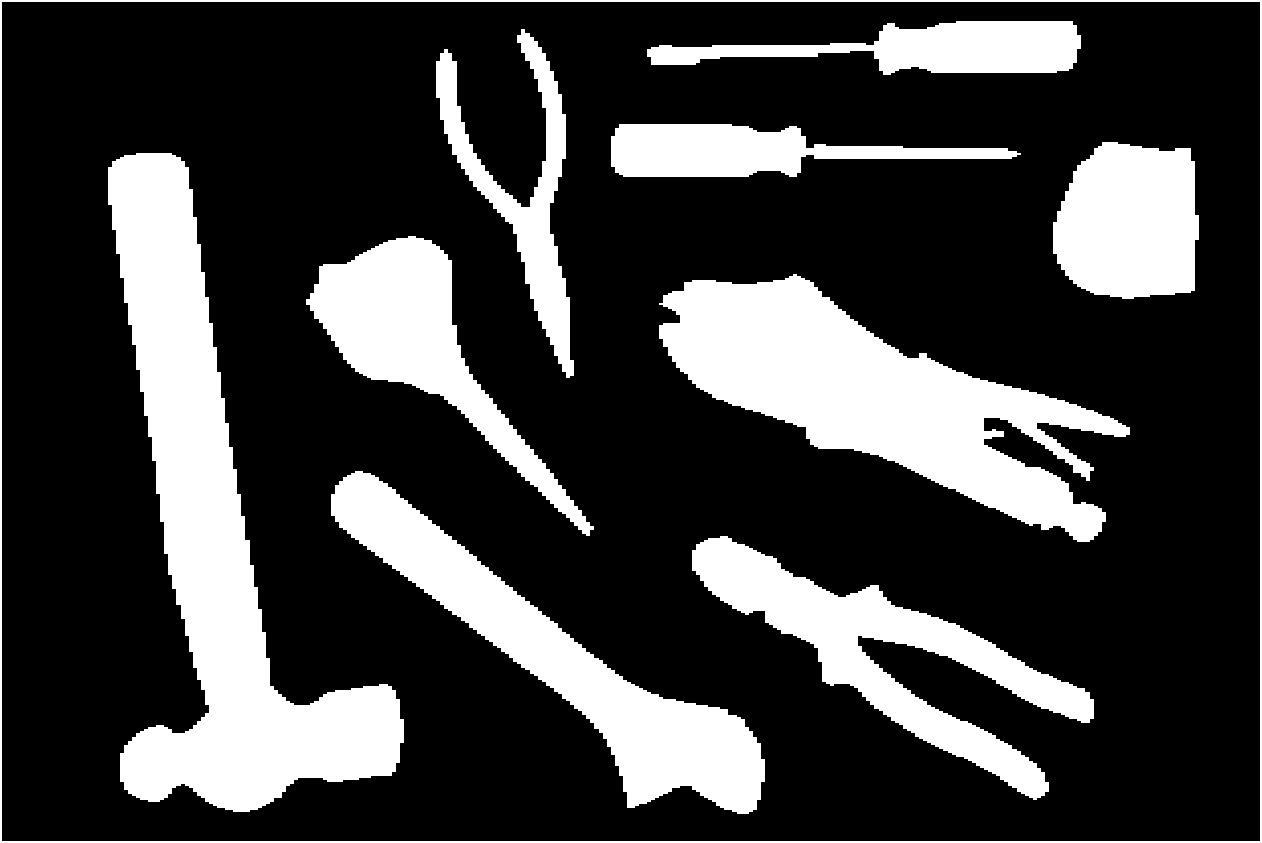
\includegraphics[width=\linewidth]{paso9}
    \caption{Imagen segmentada}
    \label{fig:1a}
  \end{subfigure}\hfill
  \begin{subfigure}{0.5\linewidth}
    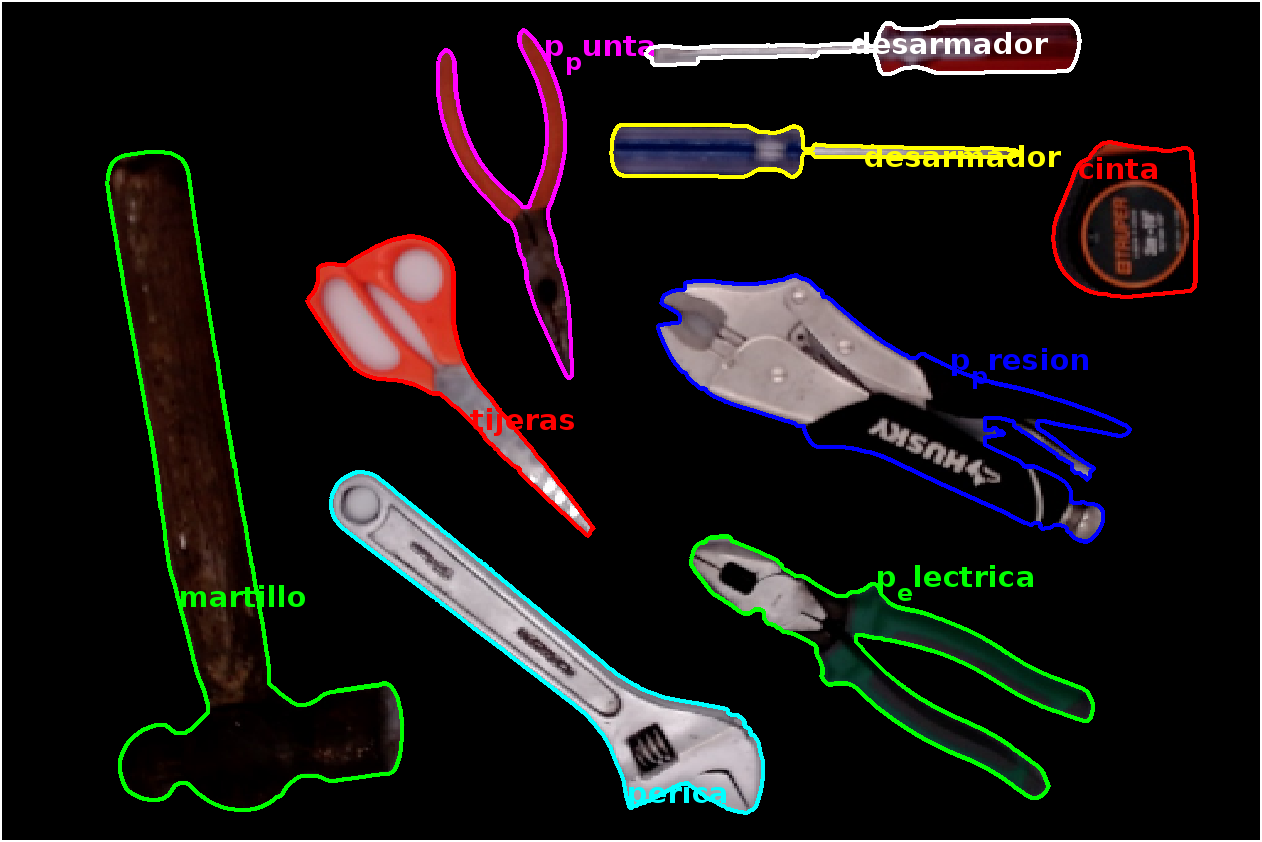
\includegraphics[width=\linewidth]{paso10}
    \caption{Imagen binaria enmascarda con los objetos}
    \label{fig:1a}
  \end{subfigure}
  \caption{Proceso de segmentado última parte.}
  \label{fig:1}
\end{figure}


Dentro de las imágenes, la similitud de esqueletos entre la cinta, la llave perica, tijera, pinzas de punta y electrica que tienen formas similares.

La mayoria de desarmadores no tiene ramas y tiene dos puntos finales, lo que lo confunde con una cinta al solo considerar las ramas y los puntos terminales se tiene una exactitud del 20\%, mientras al agregar el num de pixeles crece al 78\%, agregando más información como el área y perimetro la probabilidad de acierto crece aún más, presentandose valores arriba del 90\%.

\begin{figure}[h]
  \centering
  \begin{subfigure}{0.5\linewidth}
    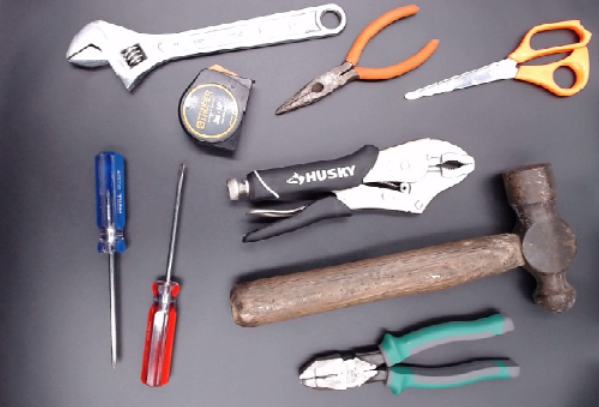
\includegraphics[width=\linewidth]{resultados_colores/todo_negro}
    \caption{Imagen objetos fondo negro}
    \label{fig:1a}
  \end{subfigure}\hfill
  \begin{subfigure}{0.5\linewidth}
    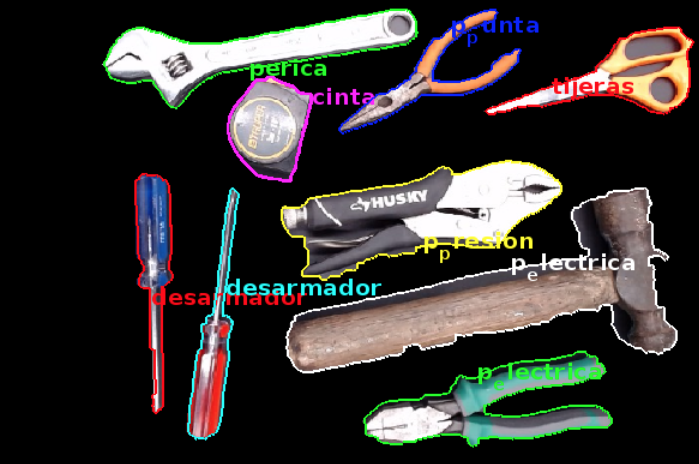
\includegraphics[width=\linewidth]{resultados_colores/resultado_negro_hue_1}
    \caption{Resultado fondo negro, hue 100\%}
    \label{fig:1a}
  \end{subfigure}
  
  \begin{subfigure}{0.5\linewidth}
    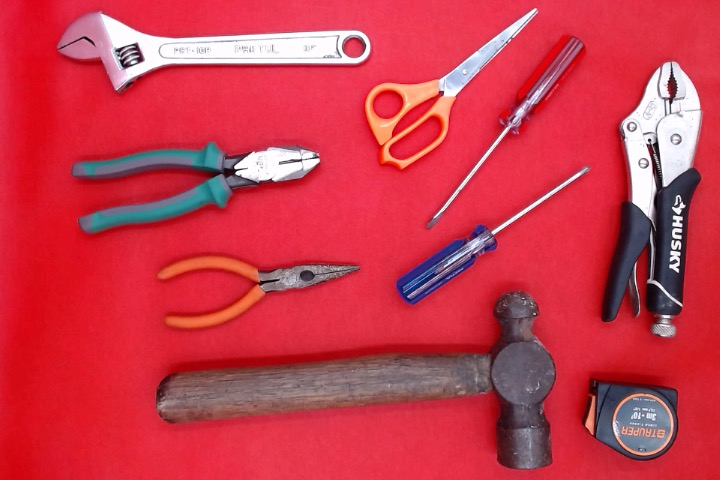
\includegraphics[width=\linewidth]{resultados_colores/todo_rojo}
    \caption{Imagen objetos con fondo rojo}
    \label{fig:1a}
  \end{subfigure}\hfill
  \begin{subfigure}{0.5\linewidth}
    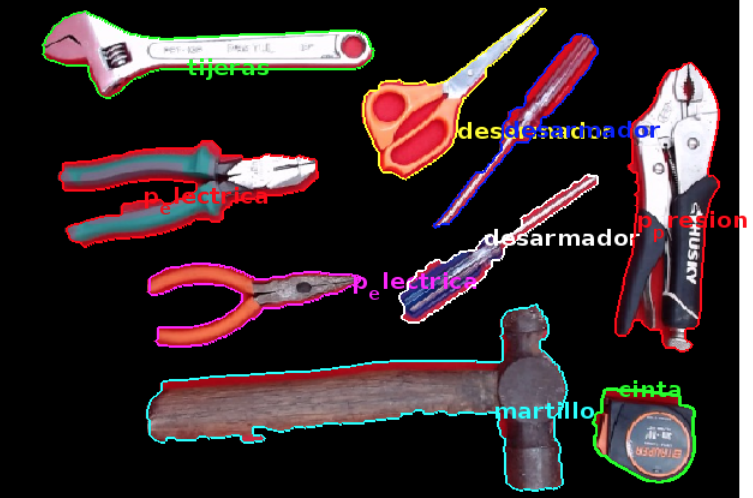
\includegraphics[width=\linewidth]{resultados_colores/resultado_rojo_cconvexo_0_89}
    \caption{Resultado fondo rojo, cerco convexo 89\%}
    \label{fig:1a}
  \end{subfigure}
  \caption{Imágenes diferentes fondos.}
  \label{fig:1}
\end{figure}

\begin{figure}[h]
  \centering
  \begin{subfigure}{0.5\linewidth}
    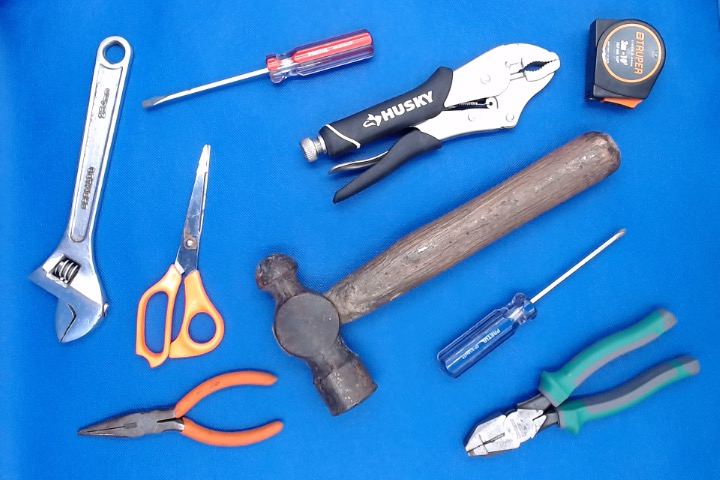
\includegraphics[width=\linewidth]{resultados_colores/todo_azul}
    \caption{Imagen objetos fondo azul}
    \label{fig:1a}
  \end{subfigure}\hfill
  \begin{subfigure}{0.5\linewidth}
    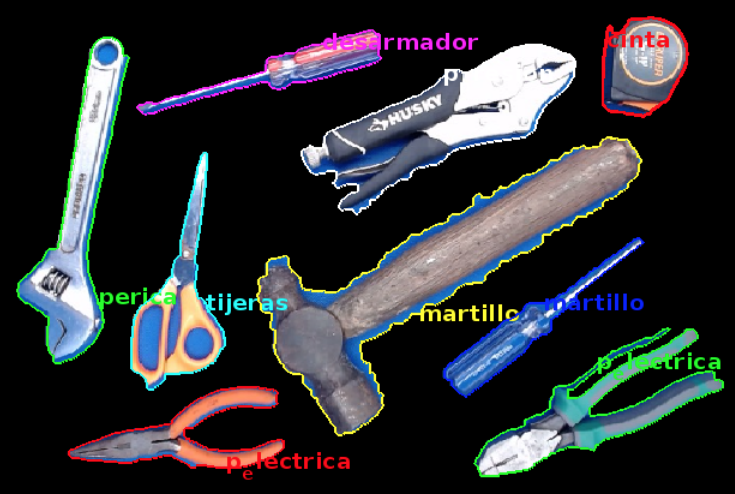
\includegraphics[width=\linewidth]{resultados_colores/resultado_azul_geom_0_97}
    \caption{Resultado fondo azul, rasgos geometricos 97\%}
    \label{fig:1a}
  \end{subfigure}
  
  \begin{subfigure}{0.5\linewidth}
    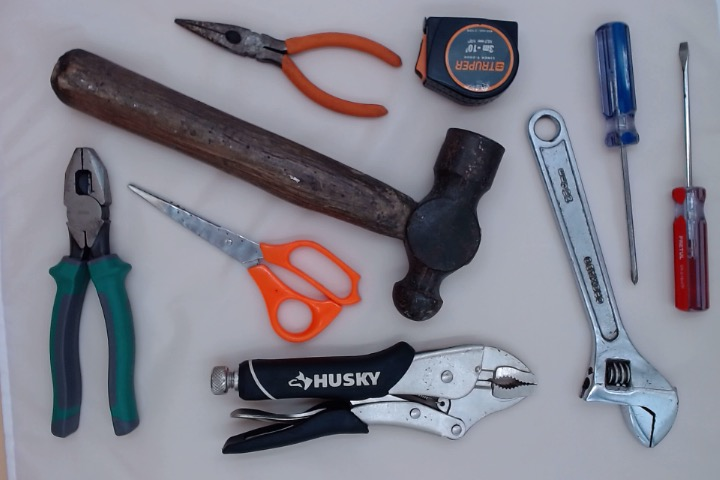
\includegraphics[width=\linewidth]{resultados_colores/todo_claro}
    \caption{Imagen objetos fondo claro}
    \label{fig:1a}
  \end{subfigure}\hfill
  \begin{subfigure}{0.5\linewidth}
    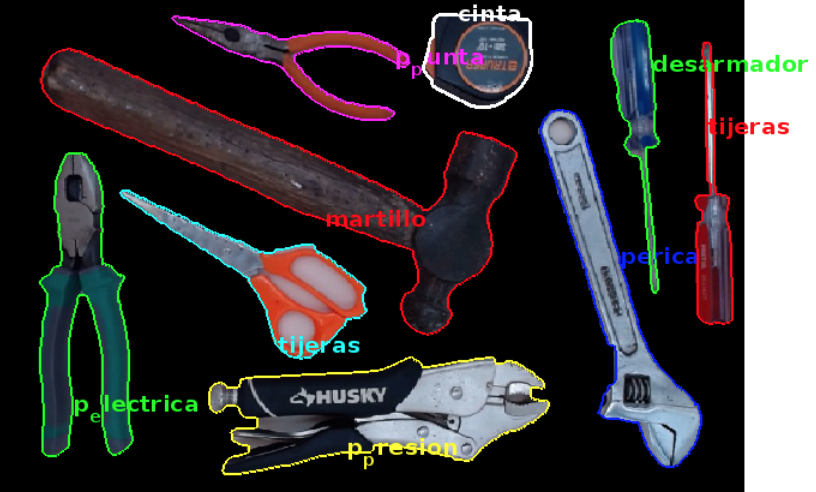
\includegraphics[width=\linewidth]{resultados_colores/resultado_claro_cconvexo_0_89}
    \caption{Resultado fondo claro, cerco convexo 89\%}
    \label{fig:1a}
  \end{subfigure}
  \caption{Proceso de segmentado última parte.}
  \label{fig:1}
\end{figure}



\newpage
\section{Conclusiones}

Estudios tempranos de Inteligencia Artificial buscaban duplicar los pensamientos humanos, pero ahora los estudios recientes muestran la tendencia en replicar el resultado y las computadoras actuan como sistemas expertos.\\

Las computadoras son dispositivos simbolicos capaces de manipular cualquier tipo de simbolos siendo los numeros una clase importante, pero las computadoras son más generales que eso. Sabemos de la generalidad de la computación desde los tiempos de Alan Touring en los 1930's y se tienen intuiciones que Babbage tuvo también estudios que fueron afirmados por Ada Lovelace, en 1842 Ada Lovelace escribió sobre la ingenieria analitica de Babbage que buscaba unir el mundo mecanico con el mundo de las cosas abstractas, en la psicologia moderna es llamado The physical symbol system hypothesis y son las bases en que la Inteligencia Artificial funciona.\\

La Inteligencia Artificial como ciencia emplea el uso de computadoras para procesar conocimientos simbolicos usando métodos de inferencias logicas, en otras palabras, nos referimos a inferencia y no calculos que se piensa en el sentido tradicional, hablamos de conocimiento y no numeros como en la forma tradicional.\\
Al poner conocimiento en programas computacionales que para los humanos nos es fácil o a veces un reto intelectual y el conocimiento que le pasamos es representativo en cierta forma particular.\\

Por otra parte, los sistemas expertos basados en conocimientos son aplicables en cualquier  área en que sea especializado el conocimiento y sea rutinario la toma de desiciones, estrategias para resolver problemas, diagnosticos, .. etc.\\
Siendo de gran ayuda en un gran rango de aplicaciones, el \textbf{conocimiento medico}, en clasificación de un experto, puede estar reflejado con el funcionamiento de una red neuronal.\\

Para algun diagnostico médico ó segmentadores más fáciles, pero igual de complicados como la segmentación en imágenes para la creación de sistemas autonomos.\\

Programas que se puedan ejecutar en cualquier computadora o dispositivo que permita la ejecución de código multiplataforma como python ó C++, que tienen capacidades altas de manipulación simbolica, la toma de desiciones es primordial en una inteligencia basada en conocimiento y esa manipulación simbolica es necesaria.

\section{Apendice}

\subsection{Script de rasgos}

La obtención de rasgos se realizó mediante un script que itera entre todas las carpetas de las imágenes, haciendo rotaciones y traslaciones aleatorias, buscando mantener la imagen, por lo que se le añade un efecto para que el fondo se replique


\begin{lstlisting}[style=Matlab-editor, caption=Script de rasgos]
%% Sample Matlab code
!mv test.txt test2.txt
A = [1, 2, 3;... foo
     4, 5, 6];
s = 'abcd';
for k = 1:4
  Disp(s(k)) % bar
end
%{
create row vector x, then reverse it
%}
x = linspace(0,1,101);
y = x(end:-1:1);
\end{lstlisting}


\subsection{Script de data aumentation}

We did some experiments \ldots

\begin{lstlisting}[style=Matlab-editor, caption=Python example]
%% Sample Matlab code
!mv test.txt test2.txt
A = [1, 2, 3;... foo
     4, 5, 6];
s = 'abcd';
for k = 1:4
  Disp(s(k)) % bar
end
%{
create row vector x, then reverse it
%}
x = linspace(0,1,101);
y = x(end:-1:1);
\end{lstlisting}

\pagebreak

\section{Experimentando en python}

\begin{lstlisting}[language=Python, caption=experimentación python]
import numpy as np
    
def incmatrix(genl1,genl2):
    m = len(genl1)
    n = len(genl2)
    M = None #to become the incidence matrix
    VT = np.zeros((n*m,1), int)  #dummy variable
    
    #compute the bitwise xor matrix
    M1 = bitxormatrix(genl1)
    M2 = np.triu(bitxormatrix(genl2),1) 

    for i in range(m-1):
        for j in range(i+1, m):
            [r,c] = np.where(M2 == M1[i,j])
            for k in range(len(r)):
                VT[(i)*n + r[k]] = 1;
                VT[(i)*n + c[k]] = 1;
                VT[(j)*n + r[k]] = 1;
                VT[(j)*n + c[k]] = 1;
                
                if M is None:
                    M = np.copy(VT)
                else:
                    M = np.concatenate((M, VT), 1)
                
                VT = np.zeros((n*m,1), int)
    
    return M
\end{lstlisting}

\begin{lstlisting}[language=Python, caption=Python example]
import numpy as np
    
def incmatrix(genl1,genl2):
    m = len(genl1)
    n = len(genl2)
    M = None #to become the incidence matrix
    VT = np.zeros((n*m,1), int)  #dummy variable
    
    #compute the bitwise xor matrix
    M1 = bitxormatrix(genl1)
    M2 = np.triu(bitxormatrix(genl2),1) 

    for i in range(m-1):
        for j in range(i+1, m):
            [r,c] = np.where(M2 == M1[i,j])
            for k in range(len(r)):
                VT[(i)*n + r[k]] = 1;
                VT[(i)*n + c[k]] = 1;
                VT[(j)*n + r[k]] = 1;
                VT[(j)*n + c[k]] = 1;
                
                if M is None:
                    M = np.copy(VT)
                else:
                    M = np.concatenate((M, VT), 1)
                
                VT = np.zeros((n*m,1), int)
    
    return M
\end{lstlisting}

\pagebreak

\bibliographystyle{abbrv}
\bibliography{referencias}  % need to put bibtex references in references.bib 
\end{document}
